\section{Identificação}
\tikzstyle{every picture}+=[remember picture]

\begin{frame}{}
  \note{
    \begin{itemize}
    \item Caixa preta, não se conhece a planta
    \item Observar sinais de entrada e saida do controlador
    \item criar modelo a partir deles 
    \end{itemize}
  }

\only<1>{ 
\begin{figure}[H]
  \centering\small
     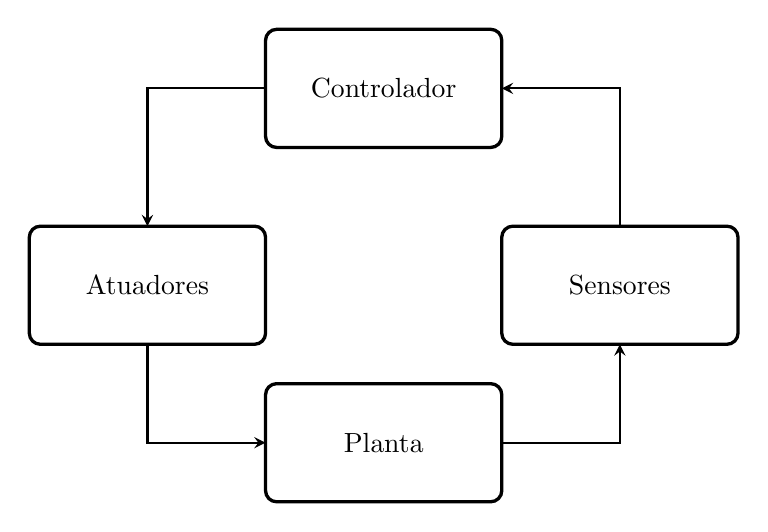
\begin{tikzpicture}
        % \draw[help lines,xstep=1,ystep=1] (0,0) grid (10,10);
        % \foreach \x in {0,1,...,10} { \node [anchor=north] at (\x,0) {\x}; }
        % \foreach \y in {0,1,...,10} { \node [anchor=east] at (0,\y) {\y}; }
        
        \draw[very thick,rounded corners] (3.5,0) rectangle (6.5,1.5);
        \draw[very thick,rounded corners] (0.5,2) rectangle (3.5,3.5);
        \draw[very thick,rounded corners] (6.5,2) rectangle (9.5,3.5);
        \draw[very thick,rounded corners] (3.5,4.5) rectangle (6.5,6);
        \draw (5,5.25) node {Controlador};
        \draw (5,0.75) node {Planta};
        \draw (2,2.75) node {Atuadores};
        \draw (8,2.75) node {Sensores};

        % actuators to plant
        \draw[->,>=stealth, thick] (2,2) -- (2,0.75) -- (3.5,0.75);

        % controller to actuators
        \draw[->,>=stealth, thick] (3.5,5.25) -- (2,5.25) -- (2,3.5);

        % Plant to sensors
        \draw[->,>=stealth, thick] (6.5,0.75) -- (8,0.75) -- (8,2);

        % Sensors to controller
        \draw[->,>=stealth, thick] (8,3.5) -- (8,5.25) -- (6.5,5.25);

        % \draw[->,>=stealth, thick] (2,4) -- (10,4);
        % \draw[fill] (2,4) circle(.05);

        % \draw[->,>=stealth, thick] (8,4.5) -- (10,4.5);
        % \draw[fill] (8,4.5) circle(.05);

        % \draw (11.4,4.5) node {Sinais};
        % \draw (11.4,4.15) node {observados};

        % \draw (1.5,5.75) node {Saídas do Controlador};
        % \draw (8.5,5.75) node {Entradas do Controlador};

      \end{tikzpicture}
 % \begin{minipage}{1.2\wd0}
 %  \centering
 %   \usebox0
  \caption{Sinais Observados de um sistema em malha fechada.}
 % \end{minipage}
    \label{fig:obsSignals}
  \end{figure}}
\only<2>{ 
\begin{figure}[H]
  \centering\small
     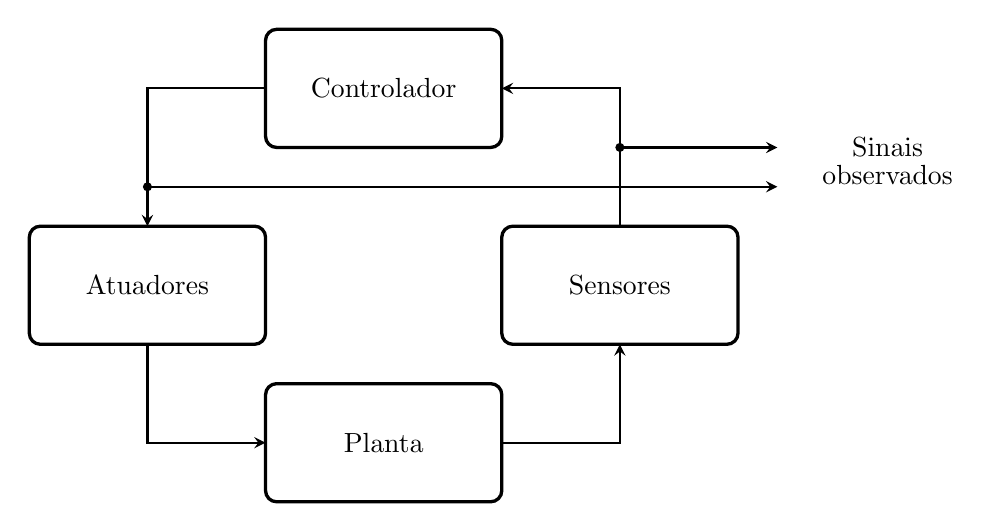
\begin{tikzpicture}
        % \draw[help lines,xstep=1,ystep=1] (0,0) grid (10,10);
        % \foreach \x in {0,1,...,10} { \node [anchor=north] at (\x,0) {\x}; }
        % \foreach \y in {0,1,...,10} { \node [anchor=east] at (0,\y) {\y}; }
        
        \draw[very thick,rounded corners] (3.5,0) rectangle (6.5,1.5);
        \draw[very thick,rounded corners] (0.5,2) rectangle (3.5,3.5);
        \draw[very thick,rounded corners] (6.5,2) rectangle (9.5,3.5);
        \draw[very thick,rounded corners] (3.5,4.5) rectangle (6.5,6);
        \draw (5,5.25) node {Controlador};
        \draw (5,0.75) node {Planta};
        \draw (2,2.75) node {Atuadores};
        \draw (8,2.75) node {Sensores};

        % actuators to plant
        \draw[->,>=stealth, thick] (2,2) -- (2,0.75) -- (3.5,0.75);

        % controller to actuators
        \draw[->,>=stealth, thick] (3.5,5.25) -- (2,5.25) -- (2,3.5);

        % Plant to sensors
        \draw[->,>=stealth, thick] (6.5,0.75) -- (8,0.75) -- (8,2);

        % Sensors to controller
        \draw[->,>=stealth, thick] (8,3.5) -- (8,5.25) -- (6.5,5.25);

        \draw[->,>=stealth, thick] (2,4) -- (10,4);
        \draw[fill] (2,4) circle(.05);

        \draw[->,>=stealth, thick] (8,4.5) -- (10,4.5);
        \draw[fill] (8,4.5) circle(.05);

        \draw (11.4,4.5) node {Sinais};
        \draw (11.4,4.15) node {observados};

        % \draw (1.5,5.75) node {Saídas do Controlador};
        % \draw (8.5,5.75) node {Entradas do Controlador};

      \end{tikzpicture}
 % \begin{minipage}{1.2\wd0}
 %  \centering
 %   \usebox0
  \caption{Sinais Observados de um sistema em malha fechada.}
 % \end{minipage}
    \label{fig:obsSignals}
  \end{figure}}
\end{frame}

\begin{frame}
  Vetores de Entrada/Saída  \note{
    \begin{itemize}
    \item armazenar os vetores de entrada e usar para
      gerar a linguagem do modelo
  \item a linguagem produzida pelo modelo deve ser o mais similar possível a
    linguagem original do sistema 
  \end{itemize}
}
\begin{equation*}
\mathbf{u}(t_1)=
\begin{bmatrix}
  i_1(t_1)&
  \dots&
  i_{m_i}(t_1)&
  o_1(t_1)&
  \dots&
  o_{m_o}(t_1)
\end{bmatrix}^T
\end{equation*}
\end{frame}
\begin{frame}{Relação entre Linguagens}
  \note{
    \begin{itemize}
    \item Linguagem original do sistema, Linguagem observada e Linguagem
      identificada
    \item preta A parte do sistema original que não foi identificada, gera
      falsos alarmes já que o que foi considerado uma falha pode estar presente
      na linguagem original do sistema mas não ter sido identificado 
    \item vermelha corresponde a parte identificada que não está presente na
      linguagem original, gera falhas não detectadas
    \item objetivo é minimizar as duas áreas 
    \end{itemize}
  }
  \begin{figure}[H]
 \sbox0{
   \includegraphics[width=0.7\textwidth]{vennDiagramLanguagesPresentation.tikz}
 }
  % \centering
 \begin{minipage}{1.2\wd0}
  \centering
   \usebox0
   \caption{Relação entre $L_{Orig}$, $L_{OrigNI}$,
    $L_{Obs}$, $L_{Exc}$ e $L_{Iden}$}.
 \end{minipage}
  \label{fig:languagesVenn}
\end{figure}
\end{frame}

\begin{frame}{Redução de Linguagens}
\begin{itemize}
\item Problema: minimizar $L_{OrigNI}$ \pause \\$L_{Orig}$ não é conhecida \pause
\item \cite{klein2005fault}:  $\exists n_0\in\mathbb{N}$ no qual
  $L_{Orig}^{\leq n_0}\backslash L_{Obs}^{\leq n_0}\approx \emptyset $  \pause \\
Considerando que $L_{Obs}\subseteq L_{Iden}$ então  $L_{Iden}^{\leq n_0}\approx
\emptyset$  \pause
\item Suposição: Todas sequências de eventos com comprimento $n_0 + 1$ são observados  \pause
\item Modelo identificado deve reduzir $L_{Exc}$ \pause
  \item \cite{moreira2018enhanced} apresentam modelo \\Derministic Automaton with
    Outputs and Conditional Transitions (DAOCT) 
\end{itemize}

\note{
\begin{enumerate}
  \item
\item Se o sistema for observado tempo o suficiente existe um número $n_0$ para
    o qual o conjunto das sequências de eventos de comprimento menor que $n_0$
    das linguagem observada e original são aproximadamente iguais
\item Neste trabalho supomos que todos eventos
\item
\item Modelo que utiliza índice de caminhos para reduzir a linguagem excedente, comparando com outros modelos da literatura
\end{enumerate}
}
\end{frame}
\begin{frame}
\begin{definition}[DAOCT]
  \label{def:daoct}
  \small
  \[ DAOCT = (X,\Sigma,f,\lambda,R,\theta, x_0,X_f)\]
  \indent X conjunto de \textbf{estados} \\
  \indent $\Sigma$ conjunto de \textbf{eventos}\\
  \indent $\Omega \subset \mathbb{N}_1^{m_i+m_o} $ conjunto de \textbf{vetores E/S}\\
  \indent $f:  X \times \Sigma^\star \rightarrow X$ função de  \textbf{transição determinística}\\
  \indent $\lambda : X \rightarrow \Omega$ função de  \textbf{saídas do stado}\\
  \indent $R = {1,2,\dots,r}$ conjunto de \textbf{indices dos caminhos}\\
  \indent $\theta : X \times \Sigma \rightarrow 2^R$ função de \textbf{estimação
    de caminho}\\
  \indent $x_0$ \textbf{estado inicial} \\
  \indent $X_f \subseteq X $ conjunto de \textbf{estados finais}
\end{definition}
\note{
\begin{enumerate}
\item usa sequências de vetores de entrada e saídas e eventos, denominados caminhos  
\end{enumerate}
}
\end{frame}


\begin{frame}{Caminhos Observados}
  \note{
\begin{itemize}
\item Os caminhos são formados por vetores e eventos
\item Os eventos caracterizam a mudança do vetor E\slash S, exemplo a bordo de
  subida de 1 ...
\end{itemize}}
  \setlength\arraycolsep{2pt}  \vspace{-0.5cm}
\small \begin{align*}
  p_1&= \left(\colvec{1\\0\\0},a,\colvec{1\\1\\0},b,\colvec{0\\1\\1},c,\colvec{0\\0\\0},d,\colvec{0\\0\\1},e,\colvec{1\\0\\0}\right) \\
  p_2&= \left(\colvec{1\\0\\0},g,\colvec{0\\0\\0},h,\colvec{1\\1\\0},b,\colvec{0\\1\\1},c,\colvec{0\\0\\0},i,\colvec{1\\0\\0},j,\colvec{0\\1\\1},l,\colvec{1\\0\\0}\right) \\
  p_3&= \left(\colvec{1\\0\\0},g,\colvec{0\\0\\0},h,\colvec{1\\1\\0},b,\colvec{0\\1\\1},i,\colvec{1\\1\\1},m,\colvec{0\\0\\0},d,\colvec{0\\0\\1},n,\colvec{1\\1\\0}\right) \\
       \end{align*}
\centering
      \only<2>{$a$ = $\uparrow$2, $b$ = $\downarrow$1$\uparrow$3, \dots} 
\end{frame}
\newcommand{\vu}{\mathbf{u}}

\begin{frame}{Caminhos Modificados}
  \note{Para diferenciar cada vetor é criada a variável livre k, que é usada
    para armazenar os $k-1$ vetores anteriores gerando caminhos modificados usando a seguinte fórmula }
\begin{equation}
  \label{eq:modifiedPath}
 p_i^k= (y_{i,1},\sigma_{i,1},y_{i,2},\sigma_{i,2},\dots,\sigma_{i,l_1-1},y_{i,l_i}) 
\end{equation}
onde 
\begin{equation}
  \label{eq:modifiedPathb}
y_{i,j}=\begin{cases}
    (\vu_{i,j-k+1},\dots,\vu_{i,j}),& \quad \text{if } k\leq j\leq l_i\\
    (\vu_{i,1},\dots,\vu_{i,j}),  & \quad \text{if } j<k
  \end{cases}
\end{equation}
\end{frame}


% http://www.texample.net/tikz/examples/beamer-arrows/
\begin{frame}{Caminhos Modificados}
  \note{
    Como que para $k=1$ são armazenados $0$ vetores anteriores, o
        modificado é igual o observado.
      } 
  \setlength\arraycolsep{2pt}
 $\bullet$ $k=2$
 \small
 \begin{align*}
   p_1&= \left(\tikz[baseline]{
            \node[anchor=base] (n1)
            {$\colvec{1\\0\\0}$};
        },a,\tikz[baseline]{
            \node[anchor=base] (n2)
            {$\colvec{1\\1\\0}$};
        },b,\tikz[baseline]{
            \node[anchor=base] (n3)
            {$\colvec{0\\1\\1}$};
        },c,\colvec{0\\0\\0},d,\colvec{0\\0\\1},e,\colvec{1\\0\\0}\right)
   \tikz[baseline] \node[coordinate] (baba) {};
\end{align*}
 \begin{align*}
  p_1^2&= \left(\tikz[baseline]{
            \node[anchor=base] (t1)
            {$\colvec{1\\0\\0}$};
        },a,\tikz[baseline]{
            \node[anchor=base] (t2)
            {$\colvec{1&1\\0&1\\0&0}$};
        },b,\tikz[baseline]{
            \node[anchor=base] (t3)
            {$\colvec{1&0\\1&1\\0&1}$};
        },c,\colvec{0&0\\1&0\\1&0},d,\colvec{0&0\\0&0\\0&1},e,\colvec{0&1\\0&0\\0&0}\right) \\ 
 \end{align*}
 \begin{tikzpicture}[overlay]
        \only<2>{\path[->,>=stealth,red] (n1) edge [bend left] (t1);}
        \only<3>{\path[->,>=stealth,red] (n1) edge [bend right] (t2);}
        \only<3>{\path[->,>=stealth,red] (n2) edge [bend left] (t2);}
        \only<4>{\path[->,>=stealth,red] (n2) edge [bend right] (t3);}
        \only<4>{\path[->,>=stealth,red] (n3) edge [bend left] (t3);}
      \end{tikzpicture}
\end{frame}


\begin{frame}{Caminhos Modificados}\note{14 vetores únicos enquanto no original com $k=1$
    só existem 6}
  \setlength\arraycolsep{2pt}
 $\bullet$ $k=2$
  \small \begin{align*}
  p_1^2&= \left(\colvec{1\\0\\0},a,\colvec{1&1\\0&1\\0&0},b,\colvec{1&0\\1&1\\0&1},c,\colvec{0&0\\1&0\\1&0},d,\colvec{0&0\\0&0\\0&1},e,\colvec{0&1\\0&0\\0&0}\right) \\ 
  p_2^2&= \left(\colvec{1\\0\\0},g,\colvec{1&0\\0&0\\0&0},h,\colvec{0&1\\0&1\\0&0},b,\colvec{1&0\\1&1\\0&1},c,\colvec{0&0\\1&0\\1&0},i,\colvec{0&1\\0&0\\0&0},j,\colvec{1&0\\0&1\\0&1},l,\colvec{0&1\\1&0\\1&0}\right) \\
  p_3^2&= \left(\colvec{1\\0\\0},g,\colvec{1&0\\0&0\\0&0},h,\colvec{0&1\\0&1\\0&0},b,\colvec{1&0\\1&1\\0&1},i,\colvec{0&1\\1&1\\1&1},m,\colvec{1&0\\1&0\\1&0},d,\colvec{0&0\\0&0\\0&1},n,\colvec{0&1\\0&1\\1&0}\right) \\
\end{align*}
\end{frame}



\begin{frame}{}
  \begin{figure}[H]
    \footnotesize
    \centering
    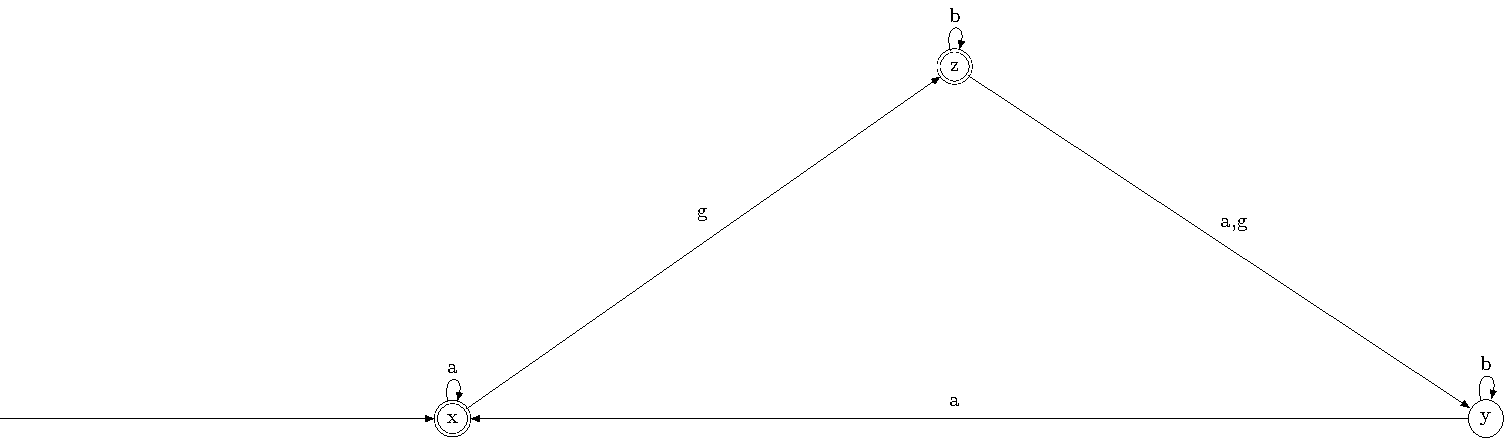
\includegraphics[width=1\textwidth]{automata/daoct/example.tikz}
  % \includetikzfigure[width=0.5\textwidth]{automata/example/example}
  \caption{Diagrama de transição de estados para $k=1$.}
  \label{fig:examplek1}
\end{figure}

\end{frame}

\begin{frame}{}
  \note{em geral aumentam o número de estados e diminuem os ciclos}
\begin{figure}[H]
    \footnotesize
  \centering 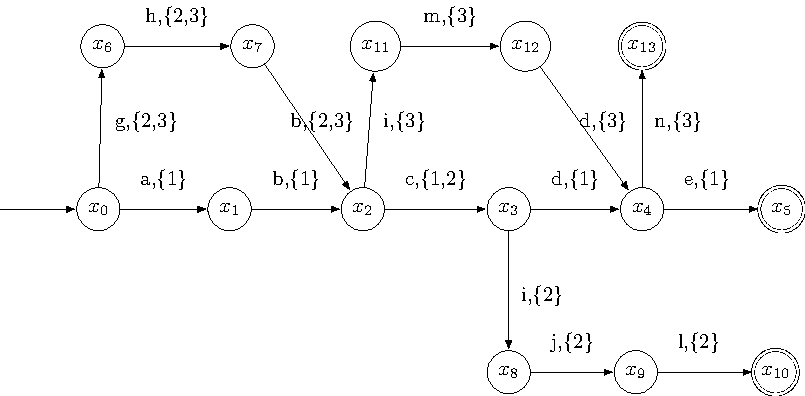
\includegraphics[width=0.9\textwidth]{automata/daoct/examplek2.tikz}
  % \includetikzfigure[width=0.5\textwidth]{automata/example/example}
  \caption{Diagrama de transição de estados para $k=2$.}
  \label{fig:examplek2}
\end{figure}
\end{frame}

%%% Local Variables:
%%% mode: latex
%%% TeX-master: "../presentation"
%%% End: